\chapter{Des atomes de Rydberg circulaires sur puce}
\label{chapter:50c}
%Excitation d'atomes de Rydberg circulaires et piégeage laser

\section{Modifications du dispositif expérimental}

\subsection{Contrôle du champ perpendiculaire à la puce}
%Second circuit de contrôle de la tension d'ionisation}

Toutes les expériences que nous décrirons dans la suite de cette thèse ayant trait au niveau $\mathrm{60S}$ ont été réalisées à l'aide de ce circuit.
Une particularité de son fonctionnement réside dans le fait que la phase d'excitation des atomes de Rydberg se fait à tension constante, et que le contrôle dynamique de la tension n'est permis que lors de la phase de détection, qui nécessite une rampe de tension comme évoqué en \ref{subsec:detection}.
Cette limitation sera corrigée plus tard par l'introduction d'un second circuit de contrôle, représenté en figure \eqref{fig:detectionbox_CdF} et son fonctionnement est détaillé ci-après.
Ce second circuit, qui permet l'application de deux rampes de tensions indépendantes pour l'excitation et la détection, a été utilisé dans toutes les expériences que nous décrirons ayant trait au niveau circulaire $\mathrm{50C}$.
%
\begin{figure}[h]
\centering
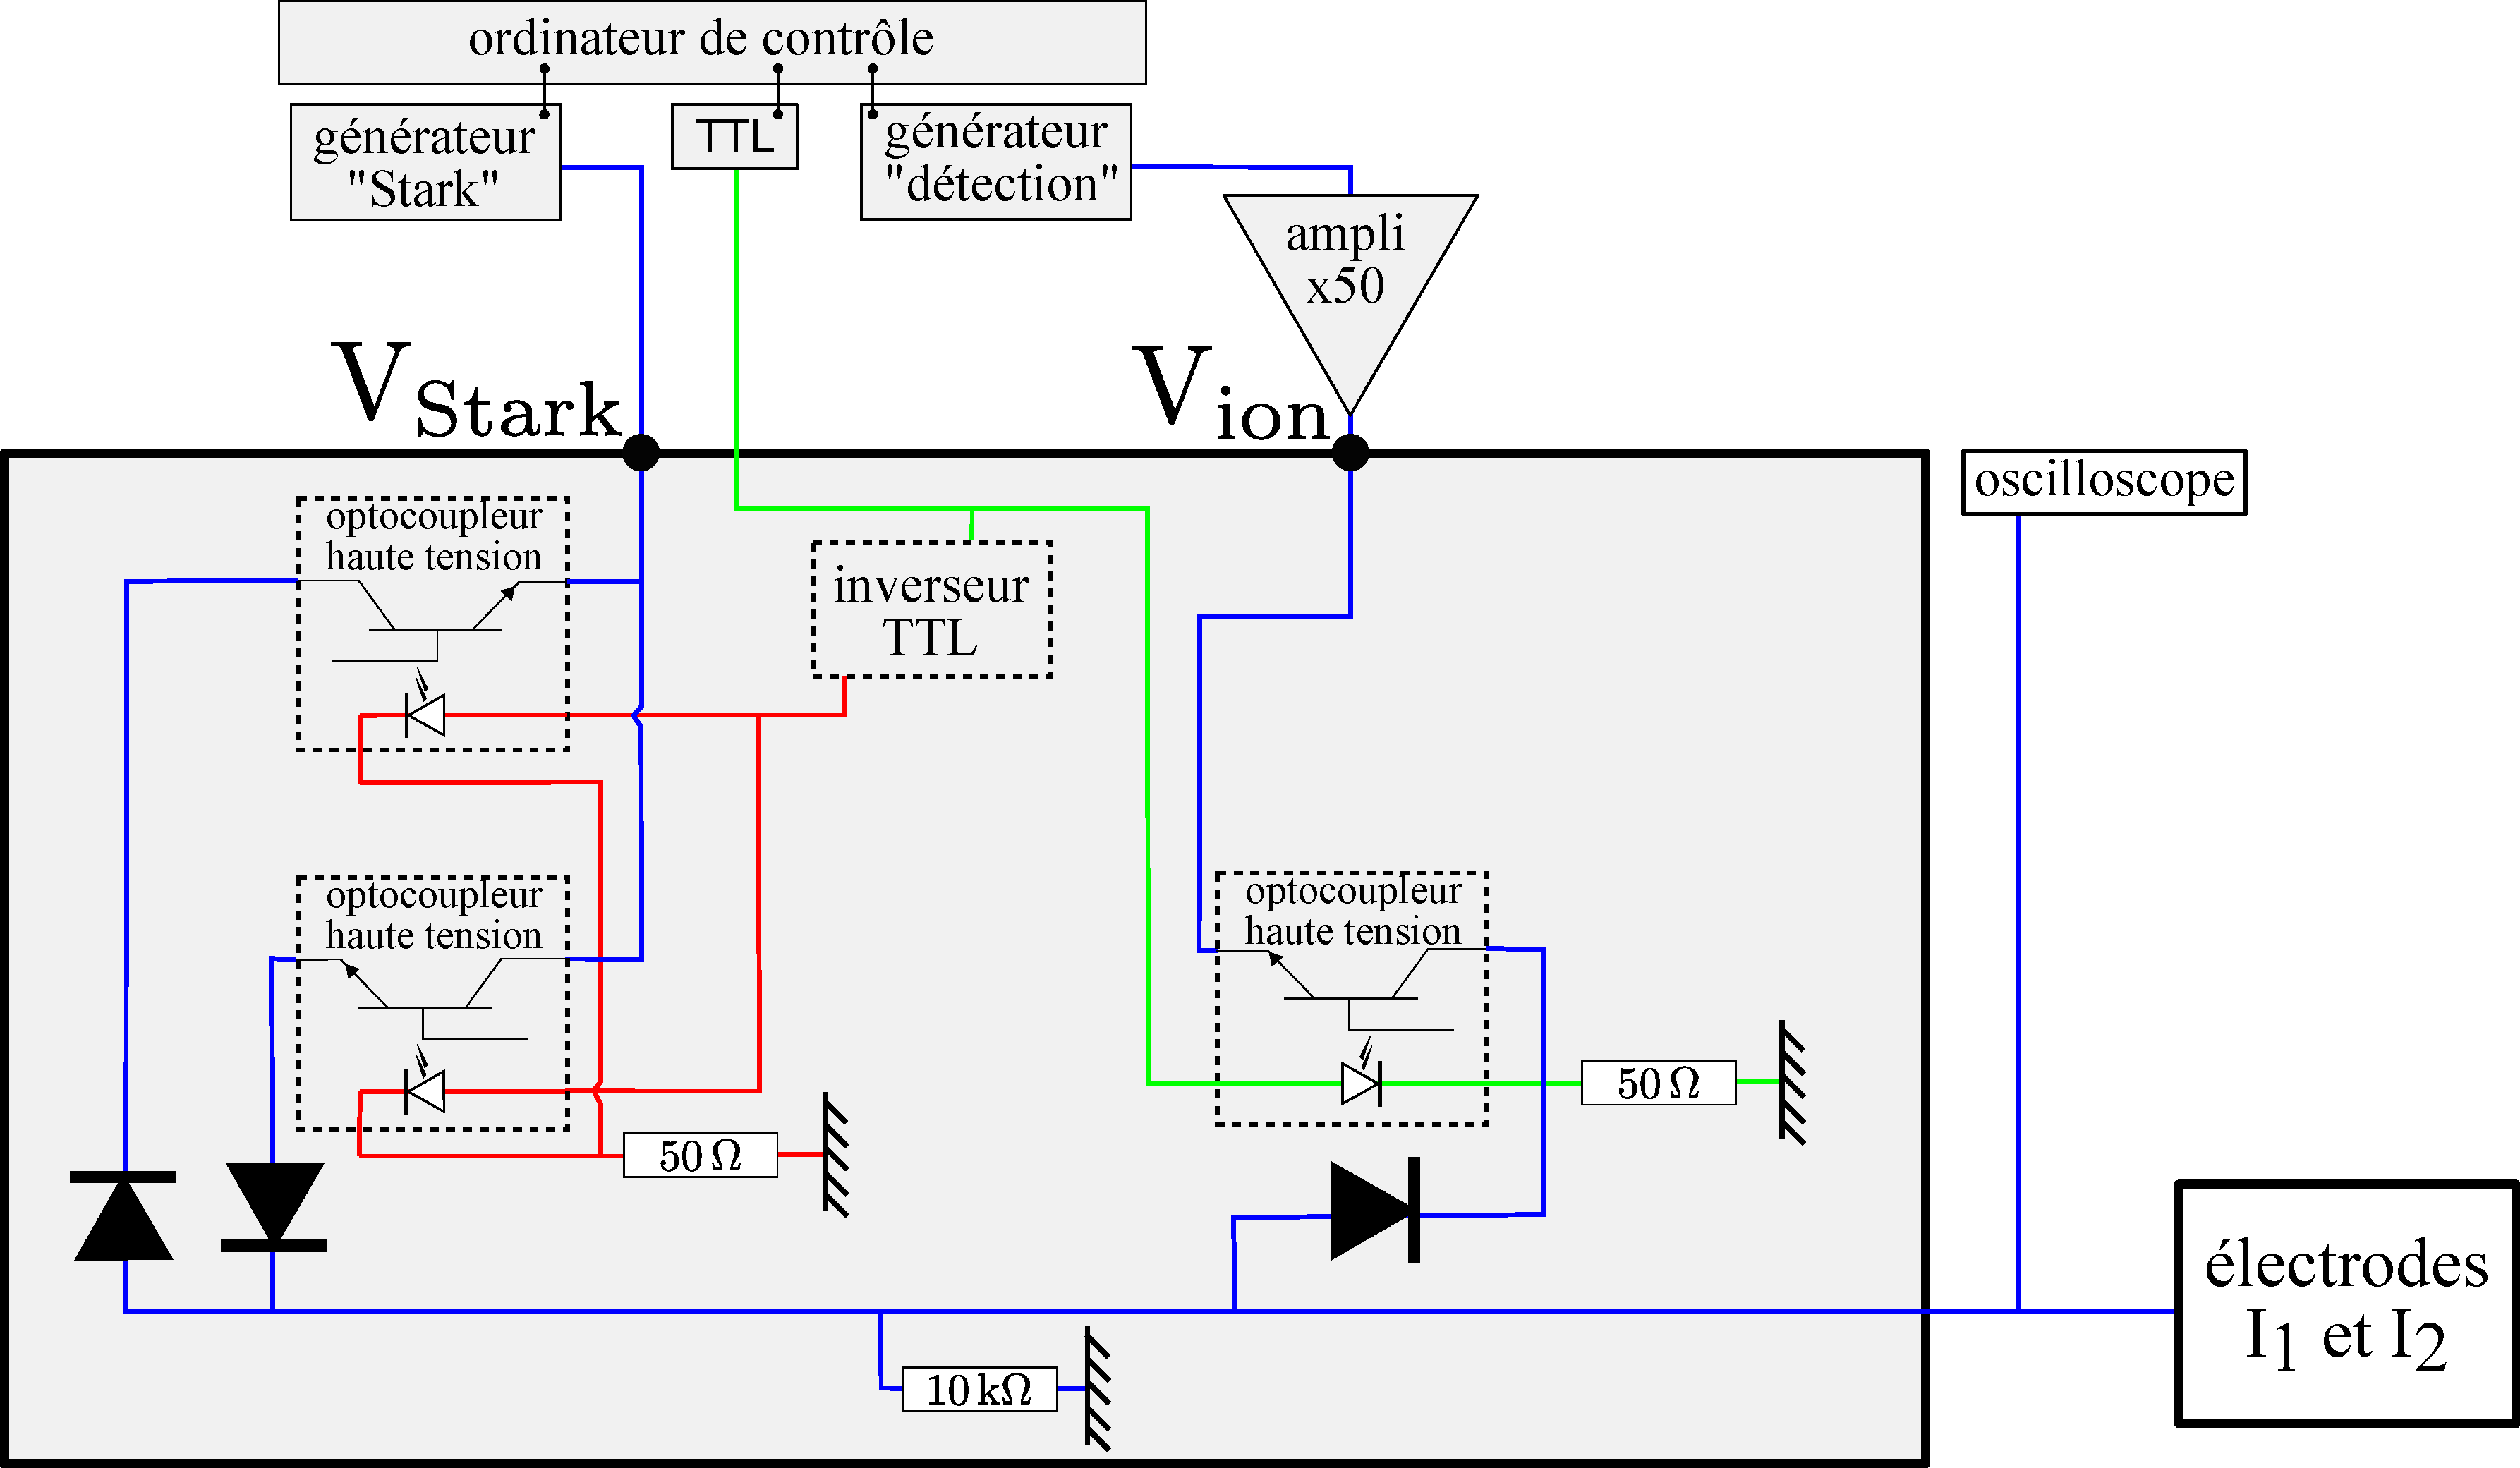
\includegraphics[width=\linewidth]{figures/setup/rydberg/detectionbox_CdF}
\caption[Second circuit de contrôle de la tension des électrodes d'ionisation]{
Second circuit de contrôle de la tension des électrodes d'ionisation.
Les tensions sont fournies par deux générateurs de fonctions arbitraires indépendants et appliquées directement aux électrodes par deux voies séparées (voie basse tension à gauche et voie haute tension à droite).
}
\label{fig:detectionbox_CdF}
\end{figure}

Dans ce second circuit de contrôle de tension, l'ordinateur de contrôle permet de programmer une rampe arbitraire sur chacun des générateurs.
La tension fournie par le générateur \og détection \fg{} est amplifiée $\num{50}$ fois et devient \og $\mathrm{V_{ion}}$ \fg{}.
$\mathrm{V_{ion}}$ est introduite dans la voie haute tension du circuit de contrôle.
La tension fournie par le générateur \og Stark \fg{} n'est pas amplifiée et est appelée \og $\mathrm{V_{Stark}}$ \fg{}.
$\mathrm{V_{Stark}}$ est introduite dans la voie basse tension du circuit de contrôle.
Pendant la phase d'excitation, le signal TTL est éteint. L'optocoupleur de la voie haute tension est alors bloquant, et les deux optocoupleurs de la voie basse tension sont passants.
L'optocoupleur du haut sert à faire passer les tension négatives et celui du bas les tensions positives.
Chacun est isolé par une diode à sa sortie, adaptée au sens de circulation du courant dans chaque voie.
La tension $\mathrm{V_{Stark}}$ est alors directement appliquée aux électrodes.
Pendant la phase de détection, le signal TTL est allumé. Les optocoupleurs de la voie basse tension deviennent bloquants et celui de la voie haute tension devient passant.
La tension $\mathrm{V_{ion}}$ est alors directement appliquée aux électrodes.
Les tensions en fin de rampe de détection peuvent aller de $\SI{-150}{\V}$ pour les niveaux voisins du $\mathrm{60S}$, et jusqu'à $\SI{-500}{\V}$ pour les niveaux voisins du $\mathrm{50C}$.
Nous avons donc conçu ce circuit de contrôle en conséquence, en utilisant des optocoupleurs capables de bloquer des tensions élevées.

 \subsection{Contrôle du champ parallèle à la puce}% et électrodes RF de circularisation}
\noindent Les dispositifs de contrôle des champs électriques que nous venons de présenter ont une lacune majeure :
ils ne permettent de varier le champ électrique que perpendiculairement à la puce, soit dans la direction $y$.
Lorsque nous avons commencé à travailler dans l'optique d'obtenir des atomes de Rydberg circulaires, nous avons souhaité pouvoir contrôler le champ électrique parallèlement à la puce.
Cela a deux conséquences.
En premier lieu, nous serons en mesure de compenser les champs résiduels dans les directions $x$ et $z$.
En second lieu, cela permettra d'appliquer un champ électrique radio-fréquence polarisé, nécessaire à la circularisation des niveaux de Rydberg, qui sera discutée au chapitre \ref{chapter:50c}.


Notre dispositif de contrôle du champ parallèle à la puce consiste en quatre électrodes cylindriques (\og électrodes RF \fg{}) , disposées en carré autour de la zone de piégeage des atomes.
En appliquant des tensions arbitraires sur ces électrodes, nous pourrons compenser les champs résiduels dans les directions $x$ et $z$, et espérer compenser même les gradients de champ dans ces directions.
En leur appliquant des tensions oscillant à une fréquence de $\SI{230}{\MHz}$ avec des phases bien optimisées, nous pourrons générer un champ électrique radio-fréquence arbitrairement polarisé au niveau des atomes.

La figure \ref{fig:RF_ELECTRODES} montre la disposition de ces électrodes au c\oe ur du dispositif expérimental.
%
\begin{figure}[!h]
\centering
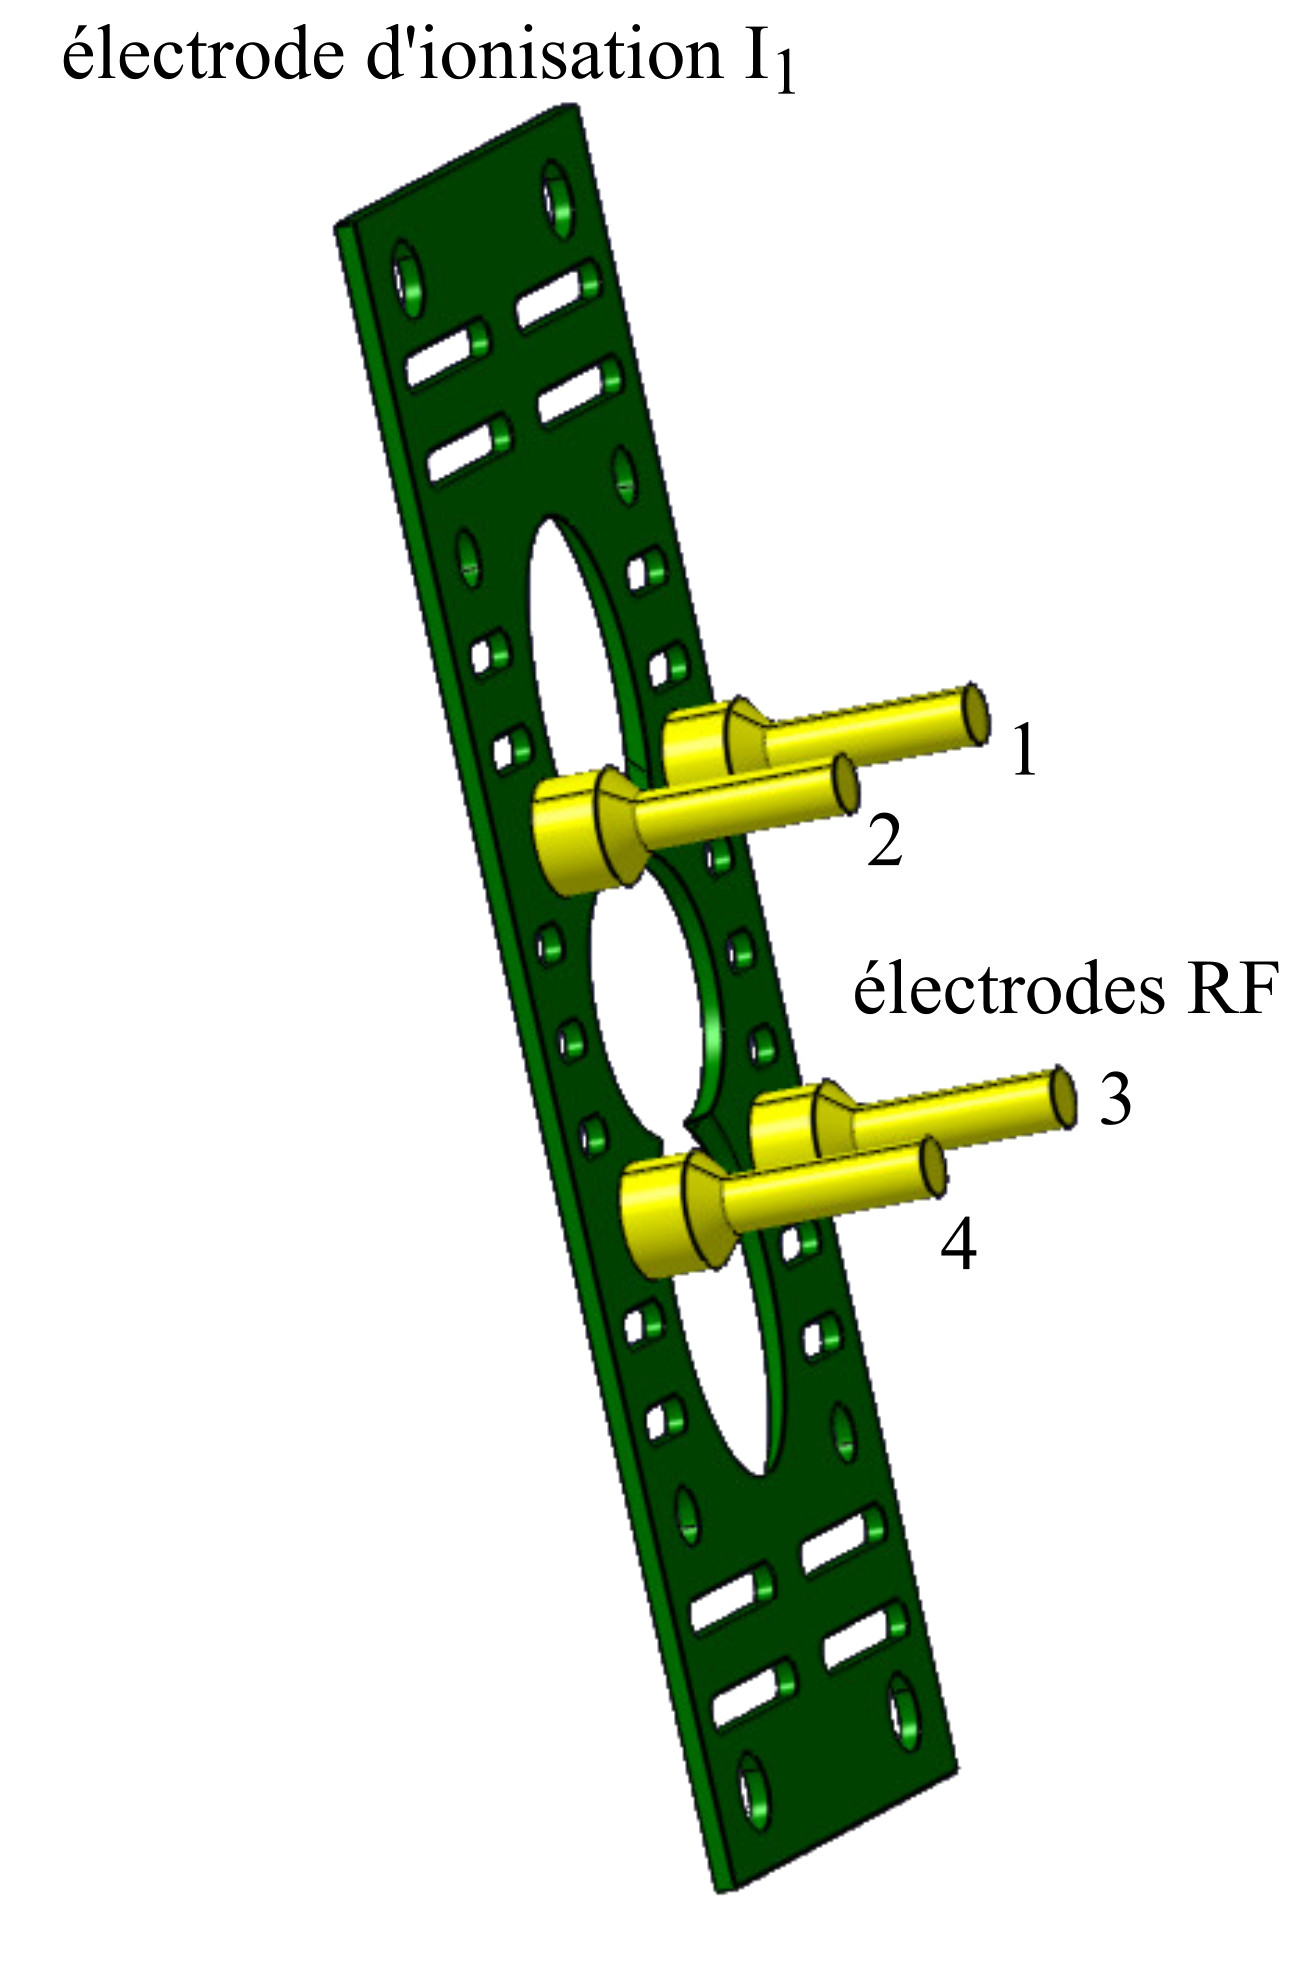
\includegraphics[width=.4\linewidth]{figures/setup/rydberg/electrodes_RF_3D_labeled.jpg}
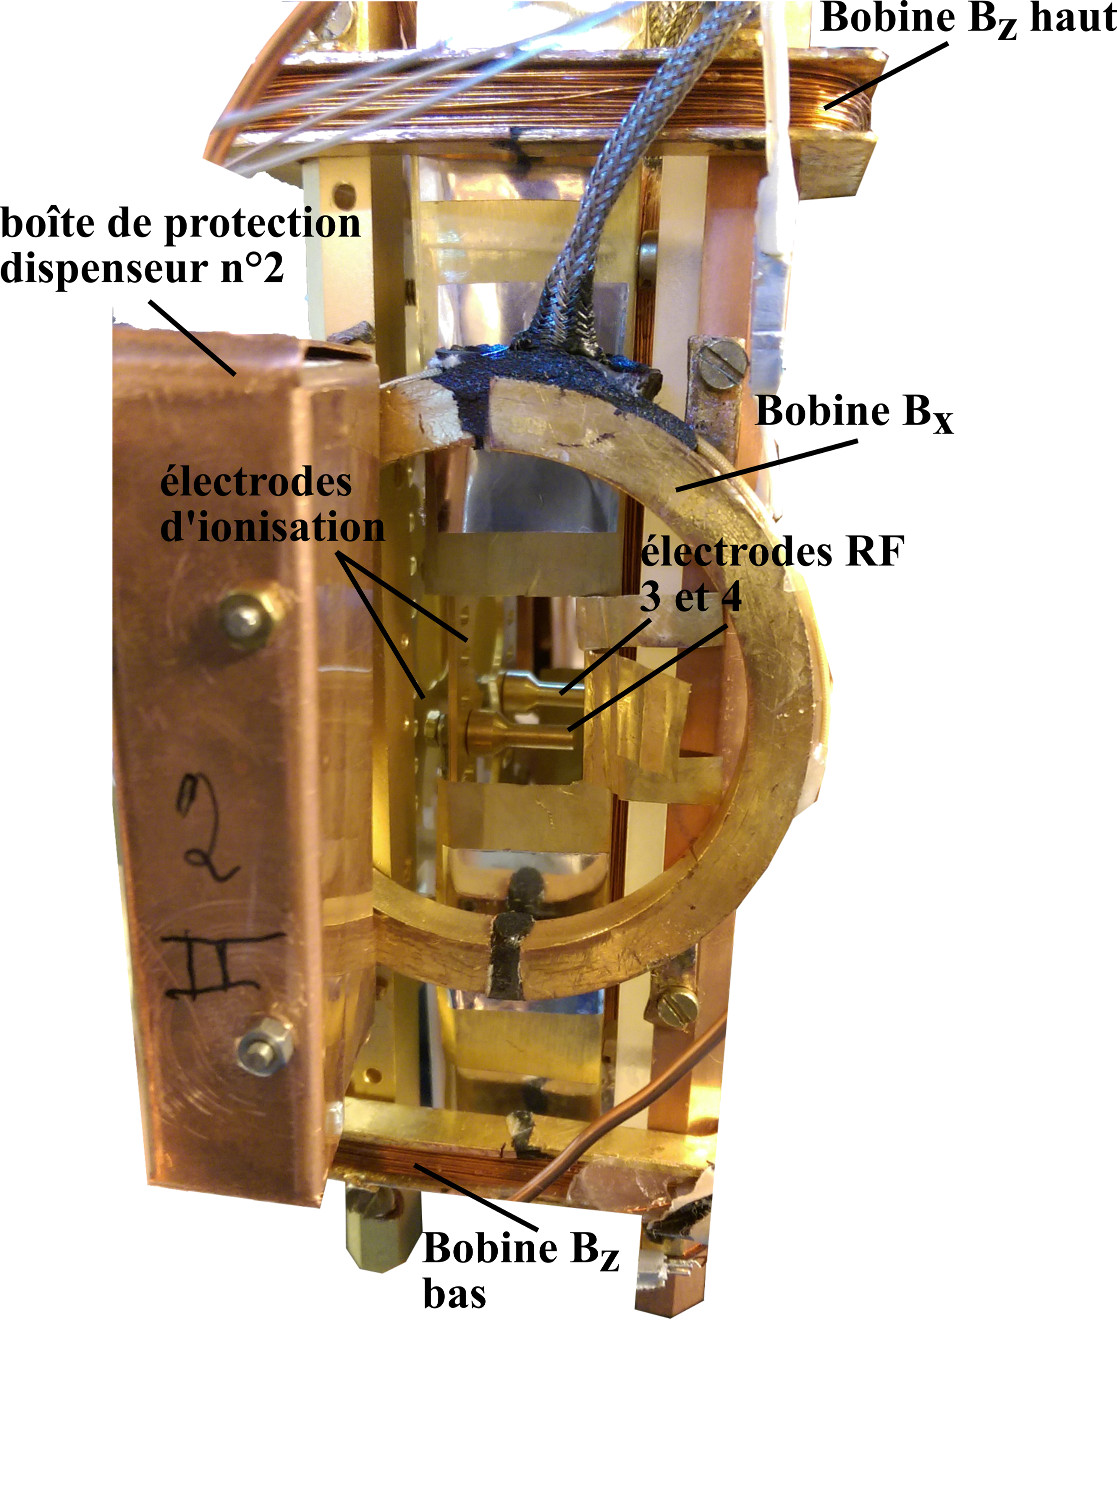
\includegraphics[width=.4\linewidth]{figures/setup/rydberg/electrodes_RF_photo}
\caption[Électrodes de circularisation et de contrôle du champ parallèle]{
Électrodes \og RF \fg{} de circularisation et de contrôle du champ parallèle à la puce.
\`A gauche, schéma représentant les électrodes RF, fixées sur l'électrode d'ionisation $I_1$, et numérotées de $1$ à $4$.
\`A droite, photographie du c\oe ur de l'expérience.
On y voit la \og boîte \fg{} de protection de l'un des dispenseurs de rubidium, les bobines de biais $B_z$ et l'une des bobines de biais $B_x$, les deux électrodes d'ionisation, et les deux électrodes RF du bas (3 et 4).
}
\label{fig:RF_ELECTRODES}
\end{figure}
%

\subsubsection*{Description technique du dispositif}
\noindent Chaque électrode RF est un cylindre de $\SI{6}{\mm}$ de diamètre et de $\SI{12}{\mm}$ de long, en cuivre doré.
Les quatre cylindres sont disposés perpendiculairement à la puce en un carré de $\SI{30}{\mm}$ de côté.
Afin de fixer les cylindres au sein du dispositif, nous avons percé des trous dans l'électrode d'ionisation $I_1$.
Chaque électrode est fixée par une tige filetée traversant l'un de ces trous et maintenue par un écrou.
Or les électrodes RF doivent être isolées de l'électrode $I_1$.
Les écrous de fixation sont ainsi isolés de $I_1$ par des rondelles en nylon.
Les tiges filetées sont quant à elles isolées par des espaceurs en céramique MACOR, logés dans la base élargie et évidée de chaque cylindre et traversant l'électrode $I_1$.
Le recouvrement de ces pièces diélectriques par les électrodes elles-mêmes est crucial, afin de limiter au maximum l'exposition des atomes à des surfaces non-conductrices susceptibles d'emmagasiner des charges électriques et de créer ainsi des champs parasites.
La longueur des cylindres en cuivre et l'épaisseur des espaceurs en céramique sont calculés pour que le bout de chaque cylindre arrive à une distance d'environ $\SI{2}{\mm}$ de la surface de la puce.

La tension appliquée à chacune des électrodes RF est amenée \textit{via} des câbles coaxiaux,  permettant de propager des signaux radio-fréquence aussi bien que des tensions constantes.
Ces câbles coaxiaux semi-rigides fins traversent le cryostat, sont thermalisés à $\SI{4.2}{\K}$ au fond de la jupe hélium.
\`A l'approche du c\oe ur de l'expérience, ils sont terminées par des connecteurs SMA, auxquels viennent se brancher des câbles plus courts et plus épais.
Cette deuxième section de câblage a deux intérêts.
Premièrement, la connexion des câbles aux cosses qui sont en contact avec les électrodes est facilitée par l'épaisseur et la solidité de ces deuxièmes câbles.
Ces cosses sont intercalées entre l'écrou de fixation de chaque électrode et un second écrou de blocage, qui garantit le contact électrique avec la tige filetée et ainsi avec l'électrode.
Deuxièmement, cela nous permet, au prix d'une simple déconnexion de connecteurs SMA, de démonter ou ajuster indépendamment les câbles coaxiaux semi-rigides et le porte-puce assorti de ses électrodes.
%La construction de ce dispositif a été l'occasion de repenser le système de fixation des électrodes d'ionisation.
%Celles-ci sont désormais fixées directement au porte-puce, par l'intermédiaire d'espaceurs métalliques isolés. Cela a permis de stabiliser le montage et la distance séparant les différents éléments.

Les tensions constantes appliquées aux électrodes sont fournies par une source analogique contrôlée par ordinateur, dont les sorties sont filtrées par un circuit RC de temps caractéristique $\tau=\SI{1}{\us}$.
Cela permet de réduire le bruit électrique de cette source à une amplitude inférieure à $\SI{5}{\milli\V}_{\mathrm{pp}}$.

\subsubsection*{Simulation du champ créé par les électrodes RF}
\noindent Il était important, afin de bien concevoir la géométrie de ces électrodes RF, de savoir quel serait l'effet des tensions appliquées dessus en termes de champ électrique au niveau des atomes.
L'estimation du champ créé ne peut pas se faire simplement par les approximations de conducteurs infinis pour lesquels il suffirait de diviser la différence de potentiel entre eux par la distance les séparant.
En effet, la géométrie des électrodes est assez éloignée de ce genre de modèle et limite ainsi déjà la validité qu'aurait une telle approximation.
De plus, la région où nous souhaitons créer du champ électrique est très proche de la puce, entre $\SI{0.5}{}$ et $\SI{2}{\mm}$ de celle-ci.
C'est-à-dire que d'une part cette région est située en dehors du volume délimité par les quatre électrodes, et d'autre part que la présence proche d'une surface conductrice considérée comme infinie (la puce) perturbera grandement les lignes de champ dans cette région.

Afin d'estimer le champ créé par les électrodes, nous avons utilisé le logiciel SIMION, destiné au calcul de potentiels et champs électriques et de trajectoires de particules chargées dans des structures arbitraires.
Les éléments que nous y avons programmés sont les suivants : la surface de la puce, les électrodes RF et les électrodes d'ionisation.
Cette structure simplifiée est représentée en figure \eqref{fig:RF_elec_SIMION}.
%
\begin{figure}[!h]
\centering
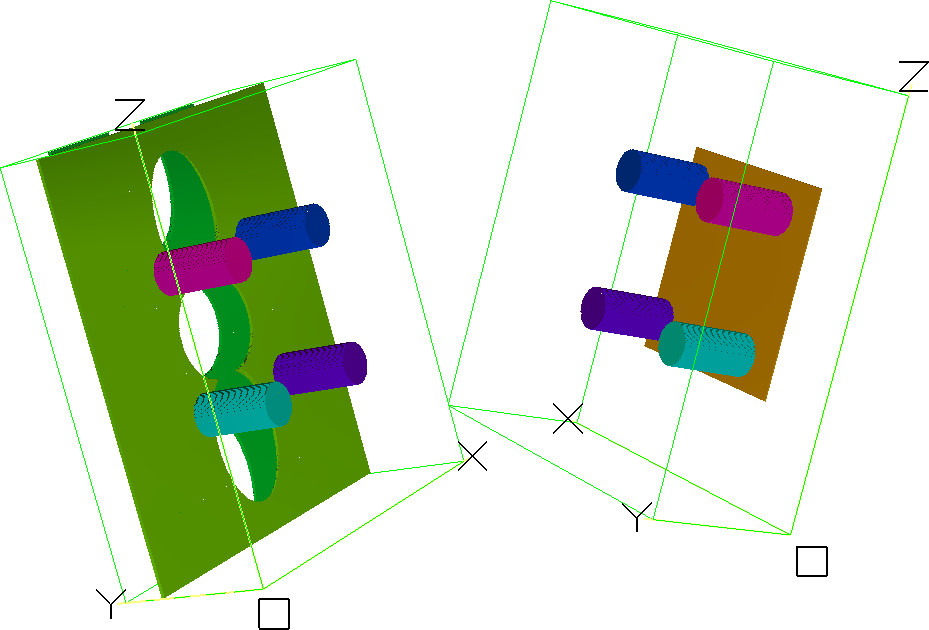
\includegraphics[width=\linewidth]{figures/setup/rydberg/RF_electrodes_Simion}
\caption[Électrodes de circularisation et de contrôle du champ parallèle]{
Électrodes \og RF \fg{} et leur environnement tels que programmés dans nos simulations SIMION.
Les quatre électrodes RF sont représentées, dans l'ordre de leur numérotation, en bleu foncé (1), rose (2), violet (3) et bleu turquoise (4).
La puce est représentée par une surface jaune, et les électrodes d'ionisation en vert clair ($I_1$) et vert foncé ($I_2$).
Les axes indiqués par les lettres $X$, $Y$ et $Z$ sont les axes que nous utilisons habituellement, bien que l'origine $O$ du repère ne soit pas la même.
Par souci de clarté visuelle, la figure de gauche représente les électrodes RF et d'ionisation sans la puce, et la figure de droite représente les électrodes RF et la puce, sans les électrodes d'ionisation.
}
\label{fig:RF_elec_SIMION}
\end{figure}
%

Nous présentons ci-dessous un exemple de simulation où l'on impose les potentiels suivants :
$\SI{+10}{\V}$ aux deux électrodes RF du haut (1 et 2), $\SI{-10}{\V}$ aux deux électrodes RF du bas (3 et 4), et $\SI{0}{\V}$ à la puce et aux électrodes d'ionisation.
%\begin{tabular}{cc}
%$10$ & $10$\\
%$-10$ & $-10$
%\end{tabular}
On espère alors appliquer un champ électrique vertical dirigé vers le bas au niveau des atomes.

La figure \eqref{fig:simion_fullregion} présente le résultat de la simulation.
%
\begin{figure}[!h]
\centering
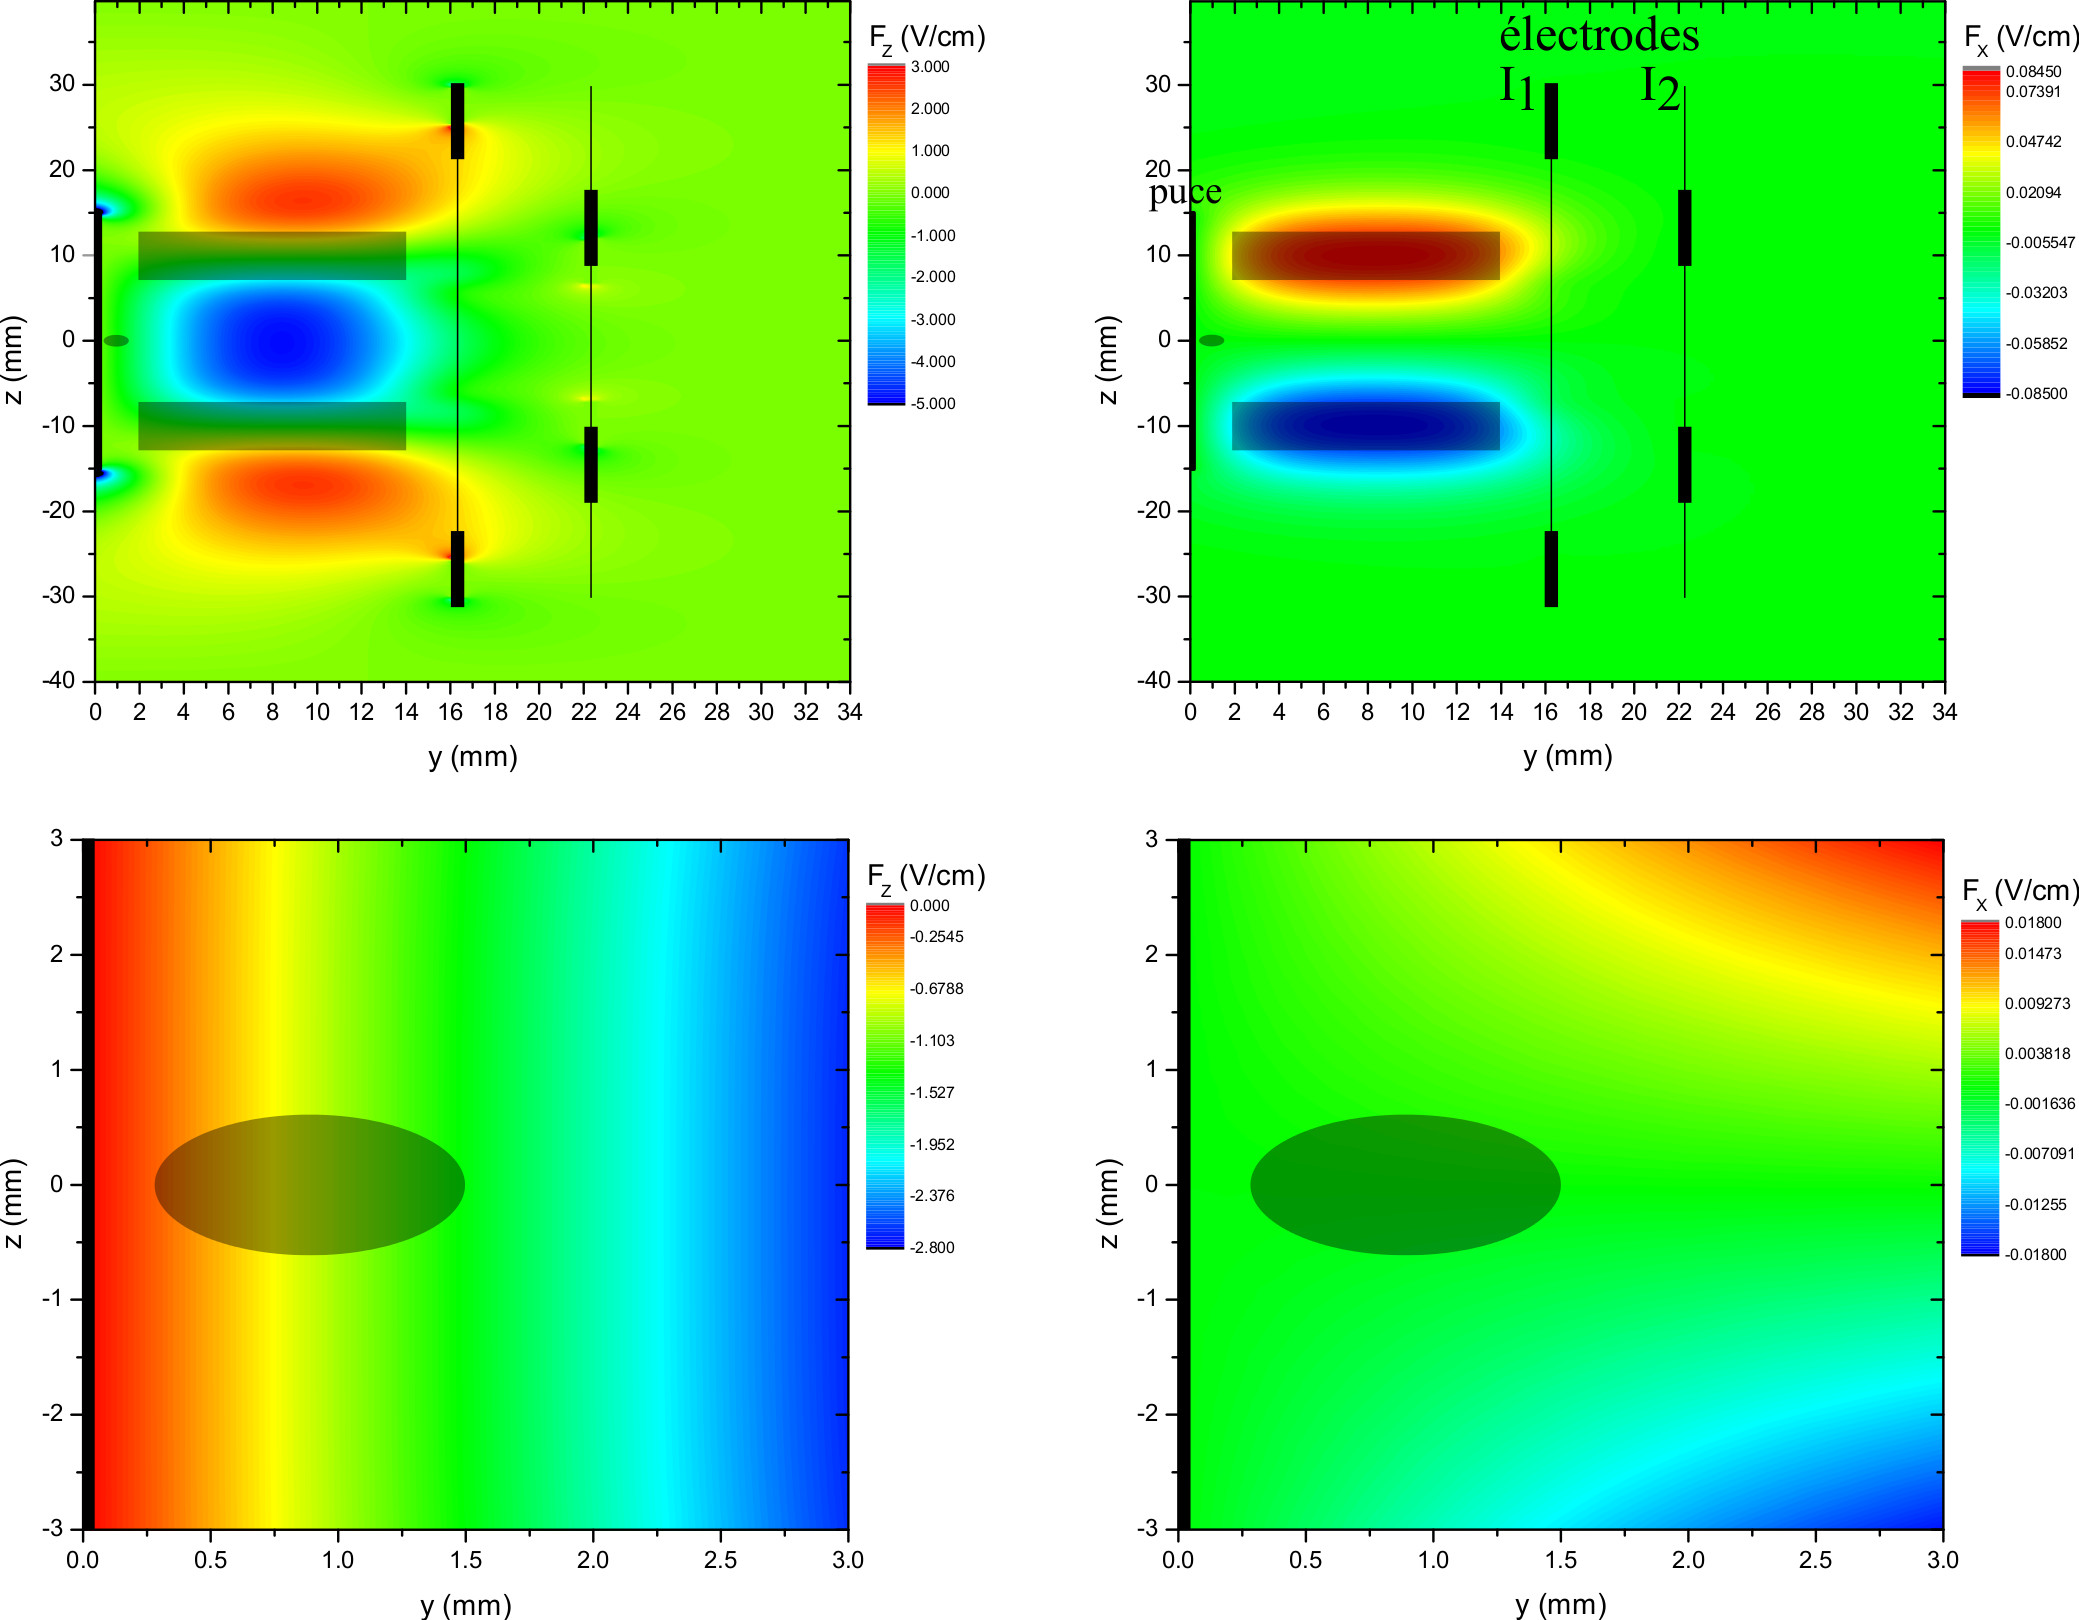
\includegraphics[width=\linewidth]{figures/setup/rydberg/simion_4quadrants}
\caption[Champ électrique créé par les électrodes RF]{
Champ électrique créé par les électrodes RF, dans le plan $(yOz),x=0$. Les échelles de longueur en $y$ et en $z$ sont différentes.
\`A gauche la composante $F_z$, à droite la composante $F_x$.
En haut, une grande région est représentée, sur laquelle sont marquées la puce et les électrodes d'ionisation(les traits épais sont les endroits où ces électrodes sont dans le plan $(x=0)$ et les traits fins sont la projection des électrodes entières sur ce plan). Les projections des électrodes RF sur le plan $(x=0)$ sont représentées en filigrane gris (rectangles), de même que la zone de piégeage des atomes (petit ovale proche de la puce).
En bas, une région beaucoup plus petite est représentée, englobant la région typique de piégeage des atomes, représentée en filigrane gris.
\`A des fins de lisibilité, les échelles de couleur sont différentes sur chacun des graphes.
}
\label{fig:simion_fullregion}
\end{figure}
%
Les deux graphes à grande échelle (en haut), permettent de confirmer que le champ créé est largement selon $z$.
En effet, la composante $F_z$ varie de $\SIrange{+3}{-5}{\V/\cm}$ lorsque la composante $F_x$ varie de $\SIrange{-0.08}{+0.08}{\V/\cm}$.
L'on retrouve le comportement idéal des conducteurs infinis dans la zone au centre des électrodes RF, autour du point $(y= \SI{8}{\mm}, z=\SI{0}{})$ : le champ y est homogène avec des valeurs de $F_z=\SI{-5}{\V/\cm}$ et $F_x=0$.
Malheureusement, nous piégeons habituellement les atomes bien plus près de la puce, à des distance comprises entre $y=\SI{0.3}{\mm}$ et $y=\SI{1.5}{\mm}$.
Il est donc important de vérifier que, dans nos régions habituelles de piégeage, notre dispositif sera suffisamment performant.
Les deux graphes à petite échelle (en bas), nous confirment cela :
nous serons capables de créer un champ de l'ordre de $F_z=\SIrange{-0.5}{-1.5}{\V/\cm}$, avec une composante $F_x$ quasi-nulle, de l'ordre du $\SI{}{\milli\V/\cm}$.

La symétrie de la structure en $x$ et en $z$ est un argument suffisant pour affirmer que nous pourrons tout aussi bien créer un champ opposé à celui-ci, c'est-à-dire avec une composant $F_z$ positive, ou encore un champ très largement orienté selon $x$.
Nous avons néanmoins occulté dans notre description un effet indésirable :
les électrodes RF créent également un champ selon $y$ dans la région qui les sépare de la puce.
Les atomes étant piégés dans cette région, délimitée par $\num{0} < y \leq \SI{2}{\mm}$, ils subiront un champ $F_y$ dû à ces électrodes.
Dans les mêmes conditions de tensions appliquées, le champ $F_y$ varie selon $z$, dans un intervalle compris entre $\SI{-0.4}{\V/\cm}$ en $z=\SI{+0.4}{\mm}$ et $\SI{+0.4}{\V/\cm}$ en $z=\SI{-0.5}{\mm}$.
Fort heureusement le champ $F_y$ reste suffisamment homogène à l'échelle de taille des nuages atomiques de diamètre $\Delta z < \SI{300}{\um}$, une taille qui est atteinte dès le stade de mélasse optique.
De plus, nous pouvons compenser sa valeur moyenne grâce aux électrodes d'ionisation, comme nous l'avons expliqué en \ref{subsec:compensation}.

Enfin, la simulation confirme que nous pourrons appliquer un champ radio-fréquence tournant dans le plan $(xOz)$ perpendiculaire à la puce, en vue de la circularisation des atomes de Rydberg sous un champ statique selon $y$.
En effet, une différence de potentiel entre les électrodes du haut (1 et 2) et celles du bas (3 et 4) crée un champ $F_z$ quasi-pur et une différence de potentiel entre les électrodes de gauche (1 et 3) et celles de droite (2 et 4) crée un champ $F_x$ quasi-pur.
Le détail des champs tournants pour la circularisation sera discuté au chapitre \ref{chapter:50c}.

%EN VRAI, MERDE ! Gros gradients de champ selon E_y quand on est près de la puce !!

Nous disposons ainsi d'un outil de contrôle du champ électrique dans toutes les directions, grâce aux électrodes d'ionisation et aux électrodes RF.


\section{Comment exciter des atomes de Rydberg circulaires}
	\subsection{Les niveaux atomiques du fondamental au Rydberg circulaire}
		\noindent schéma de niveaux et Stark maps
	\subsection{Spectroscopie 5s-50d}
		\noindent en champ nul et en champ non-nul -> choix de $m_j$
	\subsection{Spectroscopie 50d-50f}
		\noindent en champ nul et en champ non-nul -> choix de $m_l$ et problème d'élargissement Stark
	\subsection*{Le passage adiabatique}
		\noindent présenter le principe du passage adiabatique (cf Jay, Brian, Eva) et le dispositif radio-fréquence tel qu'il est chez nous

\section{Comment caractériser les atomes de Rydberg circulaires}
	\subsection{Spectroscopie microonde vers les niveaux voisins}
		\noindent 50c-51c et optimisation de la RF\\
		\noindent 50c-49c ?
	\subsection{Temps de vie}
		\noindent temps de vie théorique, temps de vie mesuré, température effective
	\subsection{Temps de cohérence}
		\noindent franges de Ramsey
	

%\section{Théorie de la force pondéro-motrice appliquée aux 50C} -> goes to chapter:circsim
%	\noindent et description du laser de piégeage

\section{Éjectable : Première évidence du piégeage des atomes circulaires}
	%\noindent chute par gravité et/ou expansion du nuage compensée par un tube de lumière
	\subsection{Dispositif laser de piégeage}
		\noindent description de l'optique de mise en forme \\
		et caractérisation du faisceau de piégeage
	\subsection{Comment observer le piégeage des atomes circulaires}
		\noindent problème du temps de vie qui empêche d'observer l'absence de chute libre \\
		\noindent comment observer un piégeage de niveaux qui ne vivent pas longtemps ? propositions envisagées\\
		premiers signaux s'ils exsitent
